\usetikzlibrary{positioning, shadows}
\begin{figure}[H]
  \centering
  \begin{tikzpicture}
    \node[inner sep=.5pt, draw=black, very thick] (step1) at (0,0)
    {
\includegraphics[width=1.5cm]{img/pipeline_1}};
    \node[inner sep=.5pt, draw=black, very thick] (step2) at (4,0)
    {
\includegraphics[width=1.5cm]{img/pipeline_2}};
    \node[inner sep=.5pt, draw=black, very thick] (step3) at (8,0)
    {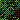
\includegraphics[width=1.5cm]{img/pipeline_3}};
    \node[inner sep=.5pt, draw=black, very thick] (step4) at (12,0)
    {
\includegraphics[width=1.5cm]{img/pipeline_4}};
    \node[draw, minimum width=1.5cm,minimum height=1.5cm, inner sep=.5pt, draw=black, very thick] (step5) at (8,-4) {?};
    \node[draw, minimum width=1.5cm,minimum height=1.5cm, inner sep=.5pt, draw=black, very thick] (step6) at (12,-4) {?};
    \node[] (m1) at (8,  -2.8) {CFA Model};
    \node[] (m2) at (12, -2.8) {RGB Model};
    \draw[->, very thick] (step1) -- node[above] {Add noise}  (step2);
    \draw[->, very thick] (step2) -- node[above] {CFA filter} (step3);
    \draw[->, very thick] (step3) -- node[above] {Demosaic}   (step4);
    \draw[->, very thick] (step3) -- node[above] {}  (m1);
    \draw[->, very thick] (step4) -- node[above] {}  (m2);

  \end{tikzpicture}
  \caption{Experiment setup}
  \label{fig:ex-setup}
\end{figure}
